\subsection{Simulação 3}

A simulação 3 consiste em um tanque de mistura, no qual estão dispostas vários sensores. Primeiramente foi descrito as entradas e saídas do sistema. 

Primeiramente foi descrito as entradas e saídas do sistema por meio das tabelas \ref{tbl:5} e \ref{tbl:6}. 

\begin{longtable}[]{@{}lcc@{}}
\toprule
Entradas & Nv. comportamental & Nv. tecnológico \\
\midrule
\endhead
Botão de partida & $LIG$ & LIG \\
Botão de parada & $NDES$ & NDES \\
Sensor de tanque vazio & \(S_{TV}\) & S\_TV \\
Sensor de tanque cheio & \(S_{TC}\) & S\_TC \\
\bottomrule
\label{tbl:5}
\end{longtable}

\begin{longtable}[]{@{}lcc@{}}
\toprule
Saídas & Nv. comportamental & Nv. tecnológico \\
\midrule
\endhead
Solenoide A & \(SOL_A\) & SOL\_A \\
Solenoide B & \(SOL_B\) & SOL\_B \\
Motor do agitador & \(M\) & M \\
\bottomrule
\label{tbl:6}
\end{longtable}


Acerca dos níveis assumidos, deixa-se claro que a chave $LIG$ é uma chave normal aberta e a chave $NDES$ (ler-se "não desligado") é uma chave normal fechada que inicia-se com nível lógico alto. Os sensores $S_{TV}$ e $S_{TC}$ assumirão nível lógico alto quando o nível de líquido alcançar eles. As saídas se comportam como na simulação 1, as válvulas solenoides abrirão quando estiverem com nível lógico alto e o motor será acionado com nível lógico alto.

Por meio da figura \ref{sim3} que ilustra o processo descrito na linguagem SFC, pode-se tirar as seguintes conclusões acerca do funcionamento das etapas.

\begin{itemize}
    \item Etapa 0 (E0):
    
    A etapa E0 configura-se como a etapa inicial. Ela marca inicio do processo e só transitará para a etapa E1 quando LIG tiver nível lógico alto;
    
    \item Etapa 1 (E1): 
    
    Quando o botão de partida for pressionado, o solenoide A será energizado, para começar a encher o tanque;
    
    \item Etapa 2 (E2): 
    
    Quando o tanque enche o sensor, nesta etapa ligará o motor do agitador por 3 min.
    
    \item Etapa 3 (E3): 
    
    Quando, o motor do agitador parar a solenoide B será ligado para esvaziar o tanque. Se o botão de parada for pressionado em qualquer momento de sistema irá parar. 
\end{itemize}

\begin{figure}[H] 
\centering
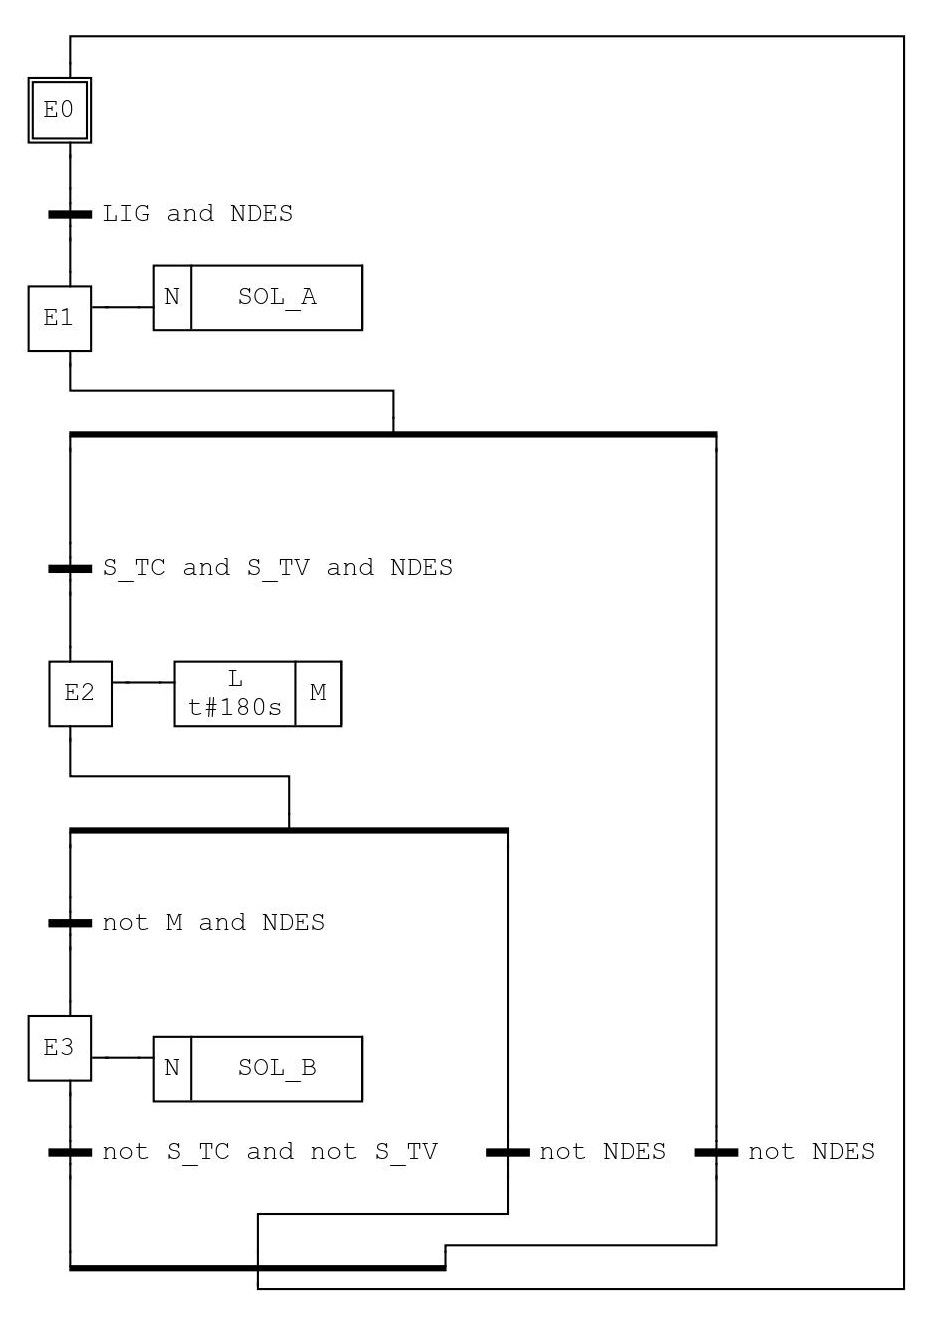
\includegraphics[width=9cm]{images/sim3.jpg}
\caption{Diagrama em SFC para a terceira simulação.}
\label{sim3} 
\end{figure}

